\section{Aufbau der Datenpakete}
\subsection{Überblick}
Es handelt sich bei dem zu entwickelnden Protokoll um ein Nachrichtenprotokoll. Daher wird der aus anderen Protokollen bekannte Begriff Datenpaket hier als eine Nachricht (Message) definiert. Diese Nachricht wird in zwei Hauptteile gegliedert. Den ersten Teil bildet der Nachrichtenheader, während der zweite Teil durch eine Instanz der Klasse \textit{Knowledge} gebildet wird.
\begin{figure}[H]
	\centering
	\hspace*{1cm}
	\makebox[\linewidth][c]{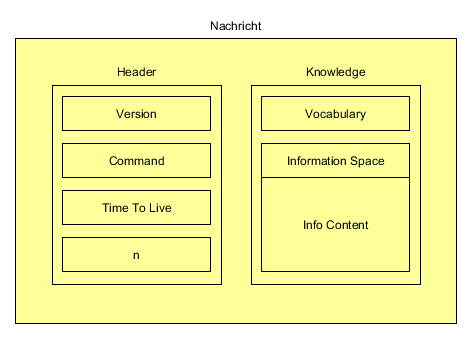
\includegraphics[width=1.0\linewidth]{entwurf/images/NachrichtAufbau1.png}}%
	\caption{Die zwei Hauptbestandteile einer Nachricht}
	\label{fig:message1}
\end{figure}
\subsection{Header}
Der Nachrichtenheader wird im Gegensatz zu anderen klassischen Routingprotokollen nicht zum Routing eingesetzt, dies ist allein von den semantischen Annotationen innerhalb des \textit{Knowledge} abhängig. Der Header ist dennoch unabdingbar, da er eine Nachricht als SharkNet Broadcast-Nachricht kennzeichnet und die Verarbeitungsart der Nachricht kennzeichnet. Der Header enthält folgende Bestandteile:
\begin{table}[H]
	\begin{center}
		\caption{Bestandteile des Headers}
		\label{tab:messageHeader}
		\begin{tabular}{l|l} 			
			Bestandteil & Erläuterung \\
			\hline
			Version & aktuelle Version des Protokolls\\
			Format & Format der Nachricht, standardmäßig JSON\\
			TTL & Time To Live Wert der Nachricht\\
			Command & Verarbeitungsart der Nachricht, Insert oder Expose\\
			Physical Sender & Absender der Nachricht\\
			Receiver Peer & Zielgerät der Nachricht\\
			Receiver Location & Ort des Absenders beim Versenden der Nachricht\\
			Receiver Time & Zeitpunkt des Absendens der Nachricht\\
			Topic & Optionales Headerthema, wird nicht vom semantischen Filter ausgewertet\\
			Type & Kennzeichnung der Nachrichtenart\\							
		\end{tabular}
	\end{center}
\end{table}
Die obligatorischen Headerbestandteile sind: Version, Format, Command, Receiver Peer und Type. Der Command ist für das Versenden der Nachrichten auf \textit{Insert} gestellt, damit die Empfangsgeräte die neue Nachricht nach erfolgreicher Filterung in ihre Wissensbasis einfügen. Der zweite Command \textit{Expose} wird fast ausschließlich von der WiFi-Komponente zum Austausch von Kontaktinformationen benutzt. Auch wenn es sich um einen Broadcast handelt, muss das Zielgerät stets im Header eingetragen sein, die Nachricht kann sonst nicht zugestellt werden. Wenn sich also beispielsweise fünf Geräte in der Nähe befinden, werden fünf Nachrichten mit angepasstem Header verschickt. Der Type markiert die Nachricht als eine Broadcast-Nachricht, damit diese nicht fälschlicherweise als Chat-Nachricht verarbeitet wird.
\subsection{Knowledge}
Der Hauptteil der Nachricht spaltet sich in drei Bereiche auf.
\begin{itemize}
	\item Das Vocabulary, welches alle Semantic Tags beinhaltet, die die Nachricht beschreiben
	\item Einen Informationsraum (InformationSpace), der die semantische Beschreibung des Nachrichteninhalts ist. Er besteht aus den in Kapitel zwei beschriebenen sieben Dimensionen mit den dazugehörigen Semantischen Netzen.
	\item Der eigentliche Nachrichteninhalt (Info Content)	
\end{itemize}
Der in Abbildung 3.1 dargestellte Bereich \textit{Info Meta Data} befindet daher sich wie oben beschrieben im Header und nicht im Knowledge.
\section{Nachrichtenaustausch}
\subsection{Ohne semantische Filterung}
Der Austausch von Nachrichten mittels des Protokolls erfolgt zunächst ungerichtet an alle Kommunikationsteilnehmer, die sich in Reichweite befinden. Jeder Teilnehmer entscheidet selbst, ob er eine Nachricht seiner Wissensbasis hinzufügt und sie ebenfalls an alle in der Nähe befindlichen Geräte sendet. Wie im Kapitel Grundlagen beschrieben, müssen dabei Loops unterbunden werden, da die Kommunikation sonst durch eine Endlosschleife fehschlagen würde. Das folgende Szenario stellt beispielhaft diese Situation ohne Beachtung einer semantischen  Filterung dar.
\begin{figure}[H]
	\centering
	\hspace*{1cm}
	\makebox[\linewidth][c]{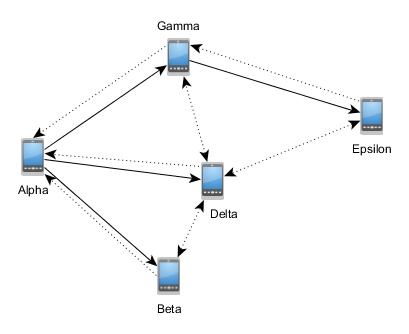
\includegraphics[width=0.6\linewidth]{entwurf/images/beispielszenario.png}}%
	\caption{Kommunikation ohne semantische Filterung}
	\label{fig:beispielszenario}
\end{figure}
Das Szenario von Abbildung 4.2 beinhaltet die fünf Smartphones Alpha, Beta, Gamma, Delta und Epsilon, welche zusammen ein kabelungebundenes Ad-hoc-Netz bilden. Der Urpsrung der Nachricht ist Alpha, welches eine Nachricht per Broadcast an alle Geräte schickt. Es befinden sich jedoch nur die Geräte Gamma, Delta und Beta in der direkten Reichweite von Alpha. Alpha sendet zunächst an alle Geräte in Reichweite die Nachricht, was jeweils durch die durchgezogene Kante symbolisiert wird. Die Geräte Gamma, Delta und Beta senden nun ihrerseits die empfangene Nachricht an alle Geräte in Reichweite. Dies würde jedoch zu Schleifen innerhalb der Kommunikation führen, falls bereits empfangene oder abgeschickte Nachrichten nicht abgelehnt werden sollten. Dies wird mit gepunkteten Kanten symbolisiert. Eine Ausnahme ist die Nachricht, die von Gamma an Epsilon geschickt wird. Da Epsilon keine Nachricht von Alpha empfangen konnte, wird die Nachricht von Gamma akzeptiert. 
\subsection{Mit semantischer Filterung}
Der Standardfall für die zu entwickelnde Anwendung wird der wiederholte Broadcast mit vorhergehender und nachfolgender semantischer Filterung sein. Jedes Gerät kann durch einen Eingangsfilter und einen Ausgangsfilter festlegen, welche Nachrichten akzeptiert und eventuell zusätzlich an andere Geräte in der Nähe weitergeleitet werden. 
\\Sollte beispielsweise Alpha eine Nachricht versenden, die nicht den Eingangsfilter von Gamma passieren kann, würde sich der eben vorgestellte Kommunikationsablauft nun wie folgt darstellen.
\begin{figure}[H]
	\centering
	\hspace*{1cm}
	\makebox[\linewidth][c]{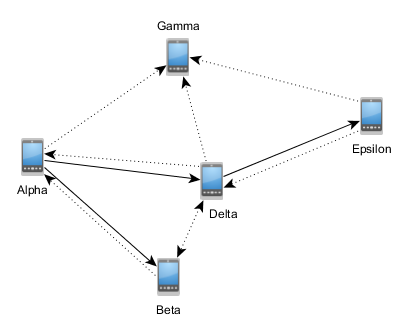
\includegraphics[width=0.6\linewidth]{entwurf/images/beispielszenario2.png}}%
	\caption{Kommunikation mit semantischer Filterung}
	\label{fig:beispielszenario2}
\end{figure}
Gamma lehnt die Nachricht aufgrund seines Filters ab, dabei ist es unerheblich von welchem Gerät die Nachricht kommt. Folglich kann Epsilon die Nachricht nicht mehr von Gamma erhalten, stattdessen wird diese nun von Delta empfangen. 
\\Falls mehrere Geräte einen restriktiven Eingangsfilter konfiguriert haben, können Nachrichten teilweise nicht an alle Geräte zugestellt werden, wie das folgende Szenario zeigt.
\begin{figure}[H]
	\centering
	\hspace*{1cm}
	\makebox[\linewidth][c]{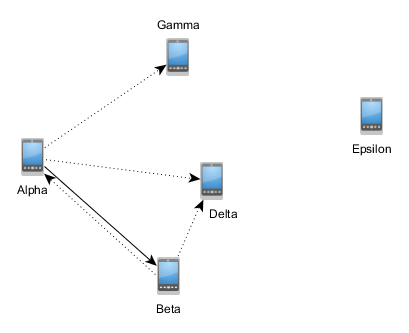
\includegraphics[width=0.6\linewidth]{entwurf/images/beispielszenario3.png}}%
	\caption{Kommunikation mit semantischer Filterung}
	\label{fig:beispielszenario3}
\end{figure}
In diesem Szenario lehnen sowohl Gamma als auch Delta die Nachricht ab, nur Beta akzeptiert die Nachricht und versucht diese weiterzuleiten. Da Epsilon sich nicht innerhalb der Sendereichweite von Alpha oder Beta befindet, kann die Nachricht das Gerät nicht erreichen. Die Anzahl der Routen wurde durch die Filterung also deutlich verringert. 
\\Dies mag zunächst problematisch erscheinen, ist aber die Intention des Protokolls. Das hier vorgeschlagene inhaltsbasierte Routing hat nicht das vorrangige Ziel, effiziente Routen zu allen Geräten zu finden, sondern soll allein von den Interessen der Geräte abhängig sein. 